\section{Findings \& Discussion of Results}
\label{sec:Fin}

\subsection{AI Score vs. Recruiter Score Correlation}
\par After responses from 4 participants, both AI and human reviewer scores calculate a pearson correlation of 0.5286 resulting in a moderate positive relationship as show in figure \ref{fig:correlation_plot}. The prototype was proven to be used as a supportive rather than replacing human reviewers. 

\begin{figure}[htbp]
    \centering
    \footnotesize \small
    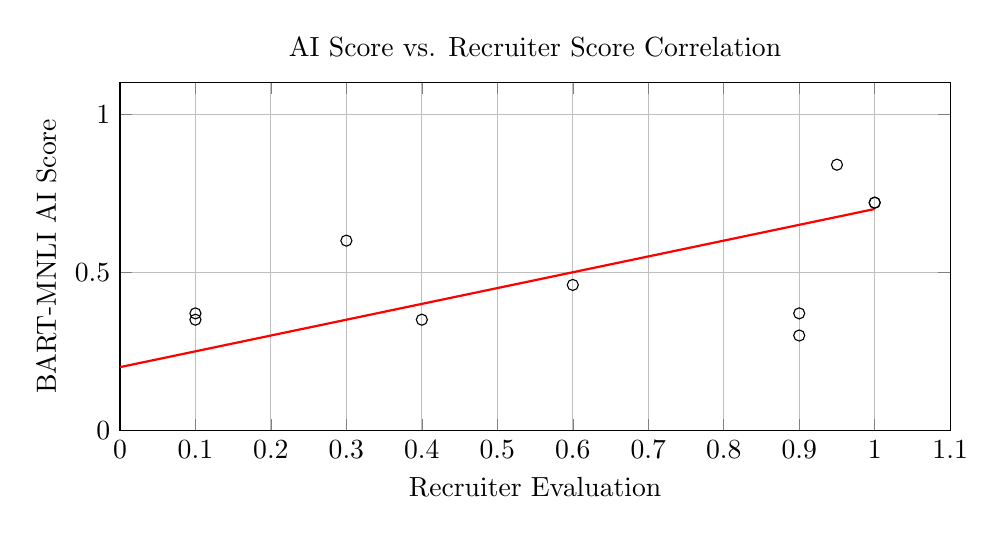
\begin{tikzpicture}
    \begin{axis}[
        width= \columnwidth,
        height= 6cm,
        title={AI Score vs. Recruiter Score Correlation},
        xlabel={Recruiter Evaluation},
        ylabel={BART-MNLI AI Score},
        xmin=0, xmax=1.1,
        ymin=0, ymax=1.1,
        grid=major,
        scatter/classes={
            a={mark=o,draw=black}}
    ]
    \addplot[
        scatter,
        only marks,
        mark size=2pt,
        scatter src=explicit symbolic
    ] table [meta=label] {
        x y label
        0.90 0.30 a
        1.00 0.72 a
        1.00 0.72 a
        0.95 0.84 a
        0.90 0.37 a
        0.40 0.35 a
        0.60 0.46 a
        0.10 0.37 a
        0.30 0.60 a
        0.10 0.35 a
    };
    % Regression Line (Approximate for r=0.52)
    \addplot [red, thick, domain=0:1] {0.5*x + 0.2};
    \end{axis}
    \end{tikzpicture}
    \caption{Scatter plot illustrating the moderate positive correlation ($r = 0.5286$) between automated and manual scoring.}
    \label{fig:correlation_plot}
\end{figure}

\par However, ZSC struggled to identify key terms found in user's open ended responses. For instance, the term 'SLA' was scored higher by the human recruiter than AI. BART-MNLI was trained on general sources such as wikipedia which possesses misunderstanding the industry context.  

\par The results align with Sikström et. al \cite{s2025sikstrom} since the source stated that Natural Language Processing is sensitive to specific word choice such as technological terms. This confirmed Sikström's theory where artifiical intelligence scoring significantly change if some words are subtle. 

\par In the session, model's confidence score dropped if the user's open response is shorter than 20 words resulting in a minimum character count. 

\begin{table}[htbp]
    \centering
    \caption{Comparative Analysis of AI vs. Recruiter Scoring for Selected Responses}
    \label{tab:Comparison}
    \resizebox{\columnwidth}{!}{% % This scales the table to fit the column
    \begin{tabular}{llp{4cm}cc} 
        \toprule
        \textbf{ID} & \textbf{Trait} & \textbf{Candidate Response} & \textbf{AI} & \textbf{Human} \\ 
        \midrule
        0 & Cons. & I managed three simultaneous projects by using a Gantt chart... & 0.72 & 1.00 \\
        \midrule
        1 & Open. & I noticed our traditional filing system was inefficient... & 0.30 & 0.90 \\
        \midrule
        2 & Extra. & I hate talking to people I don't know. I'd much rather sit in the back... & 0.30 & 0.90 \\
        \midrule
        3 & Agree. & I don't care about making friends at work. If I think an idea is stupid, I'll say it... & 0.30 & 0.90 \\
        \midrule
        4 & Neuro. & When confronted with technical debt, I focus on root-cause analysis without escalating... & 0.30 & 0.90 \\
        \bottomrule
    \end{tabular}%
    }
\end{table}

\begin{table}[htbp]
    \centering
    \caption{Operational Efficiency Comparison: AI vs. Manual Evaluation}
    \footnotesize \small
    \resizebox{\columnwidth}{!}{
    \label{tab:Efficiency}
    \begin{tabular}{|l|c|c|}
        \hline
        \textbf{Metric} & \textbf{BART-MNLI Prototype} & \textbf{Human Recruiter} \\ \hline
        Total Evaluations & 20 & 20 \\ \hline
        Avg. Time per Response & 0.35 seconds & $\sim$60.0 seconds \\ \hline
        Total Process Time & 7.04 seconds & $\sim$20 minutes \\ \hline
        \textbf{Time Reduction} & \textbf{99.4\%} & - \\ \hline
    \end{tabular}
    }
\end{table}